\documentclass[12pt]{article}

\usepackage{graphicx}
\usepackage{float}
\usepackage{hyperref}
\hypersetup{
    colorlinks=true,
    linkcolor=blue,
    urlcolor=blue,
}

%
%Margin - 1 inch on all sides
%
\usepackage[letterpaper]{geometry}
\usepackage{times}
\geometry{top=1.0in, bottom=1.0in, left=1.0in, right=1.0in}

%
%Doublespacing
%
\usepackage{setspace}
\doublespacing

%
%Rotating tables (e.g. sideways when too long)
%
\usepackage{rotating}


%
%Fancy-header package to modify header/page numbering (insert last name)
%
\usepackage{fancyhdr}
\pagestyle{fancy}
\lhead{} 
\chead{} 
\rhead{Thompson \thepage} 
\lfoot{} 
\cfoot{} 
\rfoot{} 
\renewcommand{\headrulewidth}{0pt} 
\renewcommand{\footrulewidth}{0pt} 
%To make sure we actually have header 0.5in away from top edge
%12pt is one-sixth of an inch. Subtract this from 0.5in to get headsep value
\setlength\headsep{0.333in}

%
%Works cited environment
%(to start, use \begin{workscited...}, each entry preceded by \bibent)
% - from Ryan Alcock's MLA style file
%
\newcommand{\bibent}{\noindent \hangindent 40pt}
\newenvironment{workscited}{\begin{center} Works Cited \end{center}}


%
%Begin document
%
\begin{document}
\begin{flushleft}

%%%%First page name, class, etc
Josie Thompson\\
DXARTS 200\\
13 November 2019\\

%%%%Title
\begin{center}
    In Other Words
\end{center}


%%%%Changes paragraph indentation to 0.5in
\setlength{\parindent}{0.5in}
%%%%Begin body of paper here

    \textit{In other words} is an interactive art piece about the credibility
    of news sources. The piece is meant to be part of a public setting where
    one would expect to see news. For instance, it could be in the lobby of a
    library by a bulletin board, or it could be in a main hall of a common
    building at a university. The piece itself pulls the headlines of articles
    from the front page of the Fox News Politics website and presents them on a
    screen. The viewers can then edit a word from a headline from a nearby
    interface. The code has been made open source and hosted on
    \href{https://github.com/josiest/In-Other-Words}{github}\footnotemark.

    One main goal of \textit{In other words} is to incorporate the idea of
    systems theory into the piece. \textit{In other words} acheives this in
    four distinct parts: input, output, throughput and feedback. The input to
    the piece is at first the headlines being pulled directly from the fox news
    website itself. It's in a way, like an initial condition of a differential
    equation, and furthermore like a forcing function when new articles are
    published and updated to the piece. But the central concept of the piece is
    rooted in the ability of the viewer to alter the words in these headlines.
    The output of the piece is simply the headlines that are displayed to the
    screen.

    The throughput of the piece is slightly more abstract. It is in how the
    viewer sees and reacts to the headlines and the fact that they are able to
    change them. This is where the context of the space the art piece is in
    becomes the most important factor of the piece's output. While each
    individual may react and interact uniquely with this piece, the demographic
    of the people who come into contact with it will certainly affect how the
    piece evolves over time. Finally, the feedback is in how the new words in
    the headlines change how people react to to them, and furthermore how they
    interact with them.

    This type of news-altering artwork is not an entirely new idea. This art
    piece has some similarities to
    \href{https://anthology.rhizome.org/gatt-org}{gatt.org}\footnotemark.
    \textit{gatt.org} was a fake news website made in protest to the General
    Agreement on Trade and Tariffs. It imitated the aesthetic of a government
    website, but posted articles "denouncing human rights" and "celebrating
    corporate profit (Net Art Anthology). One of the key differences between
    \textit{gatt.org} and \textit{In other words} is that \textit{In other
    words} doesn't focus on a specific political statement, but instead gives
    the audience the ability to make their own statement, although that is only
    one possible outcome.

% Use \footnotemark to make foot notes

    \begin{figure}[H]
        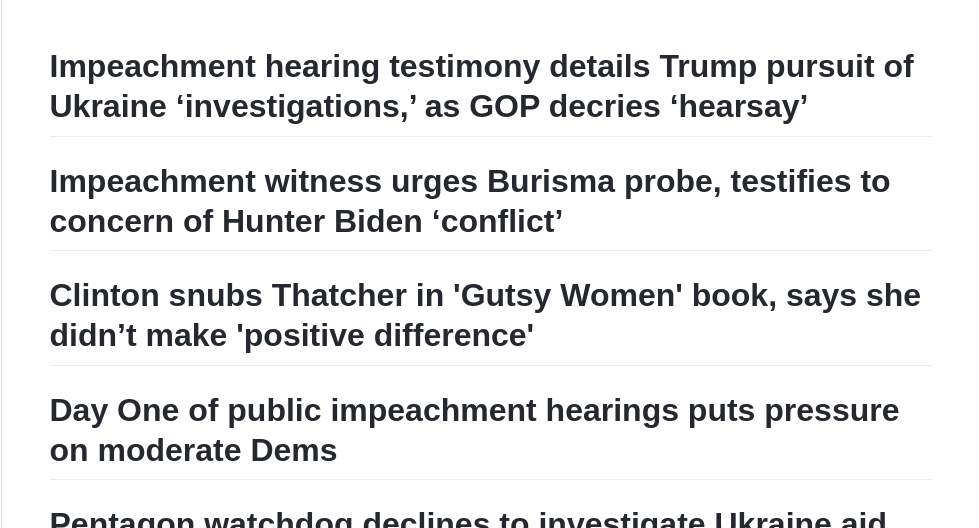
\includegraphics{ukraine.png}
        \centering
        \caption{Original headlines}
    \end{figure}
    \begin{figure}[H]
        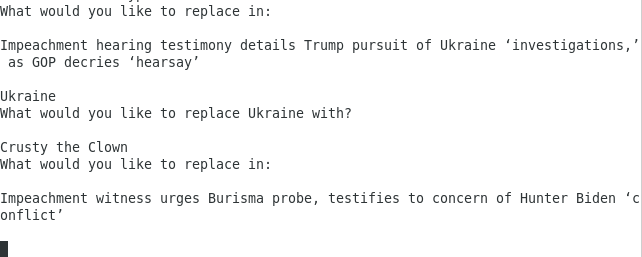
\includegraphics[width=0.75\textwidth]{input.png}
        \centering
        \caption{Interface prototype (via command line)}
    \end{figure}
    \begin{figure}[H]
        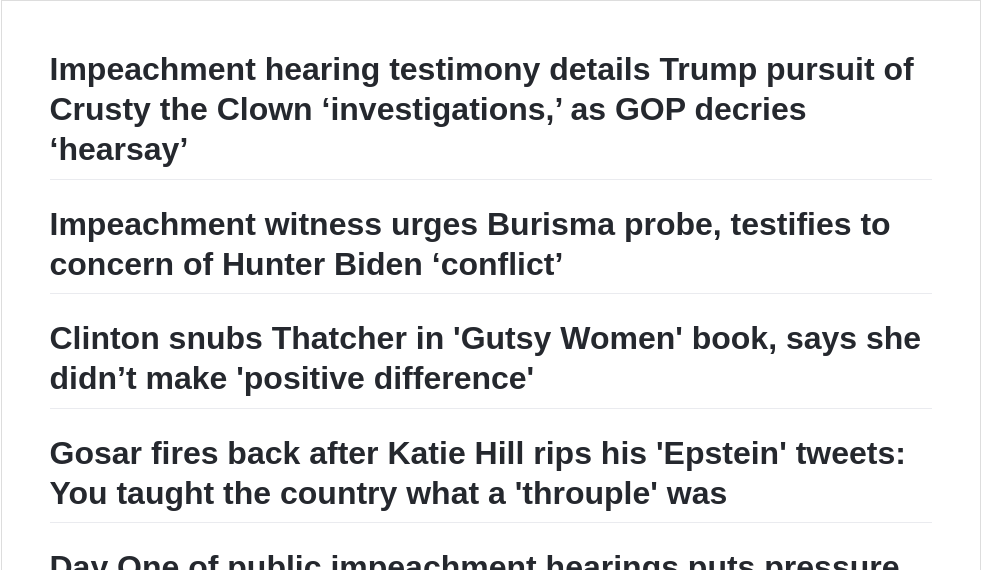
\includegraphics{crusty.png}
        \centering
        \caption{Altered headlines}
    \end{figure}

%%%%Title
\begin{center}
Notes
\end{center}


\setlength{\parindent}{0.5in}

    1. The full address for the code for \textit{In other words} is
    \url{https://github.com/josiest/In-Other-Words}.

%%%%Works cited
\begin{workscited}

    \bibent "Gatt.org." \textit{Net Art Anthology.} anthology.rhizome.org/gatt-org. Accessed 13 November 2019.

\end{workscited}

\end{flushleft}
\end{document}
\}
